\documentclass[twocolumn]{article}
\usepackage{amsmath, amssymb, graphicx, hyperref, cuted, float, comment}

\title{Seed Germination}
\author{Purva Parmar \\ 20181081}
\date{}

\renewcommand{\familydefault}{\sfdefault} 
\begin{document}
\maketitle

\graphicspath{{../Images/}}

\setlength{\parindent}{0pt}
\setlength{\parskip}{\baselineskip}
%\setlength{\columnseprule}{0.4pt}

\begin{strip}
\tableofcontents
\vspace{3em}
\end{strip}


\section{Aim}
To study germination of seeds under the influence of a designed experiment and measure the effects on root and shoot lengths.

\section{Theory}

\subsection{Germination of a Seed}

Seed Germination is the process by which a plant species grows from a seed to a plant. 

In the initial stages, the seeds take up water rapidly, resulting in swelling and softening of the seed coat at an optimum temperature. 

The seed coat then ruptures, and a primary root is formed. The seed then starts to respire and produce proteins and metabolize the stored food. 

In the final stage, the cells of the seed are elongated and divided. The cotyledons expand to form the leaves. 

Seeds need water, oxygen, an optimum temperature and light to germinate properly. Nutrients are later on needed in the soil as well.

\subsubsection{Factors affecting Seed Germination}

\begin{itemize}
    \item External Factors
    \begin{itemize}
        \item Water 
        \item Temperature 
        \item Oxygen  
    \end{itemize}
    \item Internal Factors
    \begin{itemize}
        \item Seed Dormancy \\ \\
        Under certain conditions, the seeds can be prevented from germinating even under favourable conditions.
        \begin{itemize}
        \item The seed coat is resistant to water and oxygen exchange.
        \item Seeds with undeveloped or immature embryo do not germinate.
        \item Some seeds contain plant growth regulators which inhibit seed germination.
        \item Some seeds just simply require a large amount of time for germination.
        \end{itemize}
    \end{itemize}
\end{itemize}

Cotton Wool can be used for seed germination. The soft and tender fibres, combined with water acts as a good substitute for soil.

\subsection{Statistics}

Variations are inherent in biology. We need mathematical methods to study and analyze experimental data, and to sift out the variation due to experimental manipulation from inherent variation.

There are some measures for it.

\subsubsection{Measures of central tendency}

\begin{itemize}
    \item \textbf{Mean}
    
    Mean of a data is the sum of all datapoints divided by the number of datapoints. 

    So, if the values are $x_1, x_2, \dots, x_n$, then the mean $\overline{x}$ is:

    \[
        \overline{x} = \frac{x_1 + x_2 + \dots + x_n}{n} = \frac{\displaystyle \sum_{i=1}^{n}x_i}{n}
    \]

    We represent mean of the sample by $\overline{x}$ and the mean of the population by $\mu$.

    Mean is a good measure of central tendency, however, it can be affected by outliers. A few very large or very small values can significantly affect the mean.

    \item \textbf{Median}
    
    The median of a dataset is the value that divides the dataset into two. 

    Half of the values in the data set lie above the median, and the other half lie below it.

    \item \textbf{Mode} 
    
    The mode of a dataset is the most frequent value.

\end{itemize}

\subsubsection{Variance}
There are some measures of the spread of a data. 

\begin{itemize}
    \item \textbf{Variance}
    
    The variance of a sample is denoted by $S^2$, and that of a population by $\sigma^2$. It is defined by:

    \[
        S^2 = \frac{\displaystyle \sum_{i=1}^{n} (x_i - \overline{x})^2}{n} 
    \]

    \[
        \sigma^2 = \frac{\displaystyle \sum_{i=1}^{n} (x_i - \mu)^2}{n} 
    \]

    \item \textbf{Standard Deviation}
    
    The standard deviation is the most commonly used measure of spread or measure of variation. It measures spread around the mean. 

    It is also a good indicator of outliers. It becomes useful in comparing two datasets with similar means. 

    The standard deviation of a sample is denoted by $S$ and that of a population by $\sigma$. It is defined by:

    \[
        S = \sqrt{\displaystyle \frac{\sum_{i=1}^{n} (x_i - \overline{x})^2}{n}} 
    \]

    \[
        \sigma = \sqrt{\displaystyle \frac{\sum_{i=1}^{n} (x_i - \mu)^2}{n}} 
    \]

    \begin{itemize}
        \item About 68\% of the data lies in: $\overline{x} \pm S$
        \item About 95\% of the data lies in: $\overline{x} \pm 2S$
        \item About 99\% of the data lies in: $\overline{x} \pm 3S$
    \end{itemize}
\end{itemize}

The Notation:

\begin{center}
\begin{tabular}{|c|c|c|}
\hline
& Sample & Population \\ \hline
Mean & $\overline{x}$ & $\mu$ \\ \hline
Variance & $S^2$ & $\sigma^2$ \\ \hline
Std Dev & $S$ & $\sigma$ \\ \hline
\end{tabular}   
\end{center}

\subsubsection*{Standard Error of Mean}

The Standard Error of Mean (SEM) is the expected value of standard deviation of means of several samples. 

It can be estimated from a single sample as:

\[
    \textsf{SEM} = \frac{S}{\sqrt{n}} 
\]

where $S$ is the Standard Deviation of the sample, and $n$ is the sample size. 

The Population Mean then can be represented as:

\[
    \mu = \overline{x} \pm \textsf{SEM} 
\]

\subsection{Normal Distribution}

A Normal Distribution is also called a Gaussian Distribution. It is a probability distribution that is symmetric about the mean, showing that the data near the mean are more frequent in occurence than the data far from the mean. 

It appears as a bell curve in graph form.

The Normal Distribution is motivated by the Central Limit Theorem, which states that averages calculated from independent, identically distrubuted random variables have approximately normal distributions, regardless of the type of distribution from which the variables are sampled, provided it has a finite variance. 


\[
    f(x \mid \mu, \sigma^2) = \frac{1}{\sqrt{2\pi \sigma^2}} e^{-\frac{(x-\mu)^2}{2\sigma^2}} 
\]
where\\
$\mu$ = Mean\\
$\sigma^2$ = Variance

\begin{figure}[h]
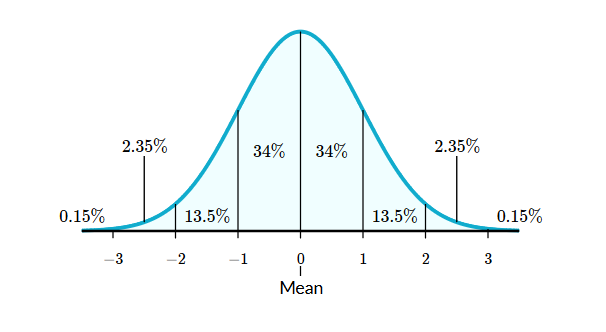
\includegraphics[width = \linewidth]{Normal Distribution Khan Academy.png}
\caption{Normal Distribution [Source: Khan Academy]}
\end{figure}


\subsection{Hypothesis Testing}

Hypothesis Testing is the use of statistics to determine the probability that a given hypothesis is true. 

The best way to determine whether a statistical hypothesis is true would be to examine the entire population.

However, this is often impractical. We study random samples from the population and if the sample data is not consistent with the statistical hypothesis, the hypothesis is rejected.

There are two types of statistical hypothesese:

\begin{itemize}
    \item \textbf{Null Hypothesis ($\sf H_{\circ}$)}: Sample observations result purely from chance. In other words, the population mean of test ($\mu_T$) is the same as population mean of control ($\mu_C$).
    
    $\sf H_{\circ}: \quad \mu_C = \mu_t$

    \item \textbf{Alternative Hypothesis ($\sf H_A$)}: Observations are influenced by some non-random cause. In other words, the population mean from test is significantly different compared to the population mean from control.
    
    $\sf H_A: \quad \mu_C \neq \mu_T$

\end{itemize}

\subsubsection{Testing Procedure}

\begin{enumerate}
    \item Formulate the \textbf{Null Hypothesis} $H_{\circ}$ and \textbf{Alternative Hypothesis} $H_A$. 
    \item Identify a \textbf{test statistic} that can be used to assess the truth of the null hypothesis.
    \item Compute the \textbf{P-value}, which is the Probability that a test statistic at least as significant as the one observed would be obtained assuming the Null Hypothesis were true. 
    
    The smaller the P-value, the stronger the evidence against the Null Hypothesis.

    \item Compare the P-value to an acceptable significance value $\alpha$ (called the \textbf{alpha value}). 
    
    If $p \leqslant \alpha$, the observed effect is statistically significant. The Null Hypothesis is ruled out and the Alternative Hypothesis is valid.
    
    Usually, $\alpha = 0.05$. 
\end{enumerate}
    
\subsubsection{Decision Errors}

\begin{itemize}
    \item \textbf{Type I Error}: Rejecting a Null Hypothesis that is actually true
    
    The probability of committing a Type I error is called the \em{significance level} or \em{alpha}, denoted by $\alpha$.

    \item \textbf{Type II Error}: Failure to reject a Null Hypothesis that is actually false. 
    
    The probability of committing a Type II Error is called \em{Beta}, denoted by $\beta$. The probability of \em{not} committing a Type II Error is called the \em{Power} of the test. 
\end{itemize}

In a nutshell,
\begin{center}
\begin{tabular}{|c|c|c|}
    \hline
    & \textbf{Accept} $\bold{H_{\circ}}$ & \textbf{Reject} $\bold{H_{\circ}}$ \\ \hline
    $\bold{H_{\circ}}$ \textbf{Correct} & \checkmark & Type I Error \\ \hline
    $\bold{H_{\circ}}$ \textbf{Wrong} & Type II Error & \checkmark \\ \hline
\end{tabular}
\end{center}

\subsubsection{Paired t-test}

The Paired t-test is used to compare means of two samples. 

\[
    \rm t = \frac{\overline{x_C} - \overline{x_T}}{\sqrt{\frac{S_C^2}{N_C} + \frac{S_T^2}{N_T}}}
\]

The numerator takes the difference between means of samples from control and test. The larger this value is, the more is the effect of the test.  

The denominator is the sum of the standard errors. 

Overall, the t-value is a normalized value which shows how significantly different is the mean of control from the mean of test. 

Larger the t-value, the more significant is the result. 

Smaller t-values indicate overlap in samples. That is, the samples may be from the same population. 

\subsubsection{ANOVA}

ANOVA stands for \textbf{Analysis of Variance}. It is a collection of statistical models and related estimation procedures to analyze the differences among group means in a sample. 

If $C$ is the control, and $T_1, T_2, \dots, T_m$ are the tests, then for ANOVA:

\begin{align*}
    \sf H_0 &= \mu_C = \mu_{T_1} = \mu_{T_2} = \dots = \mu_{T_m} \\
    \sf H_A &= \text{At least one mean is different}
\end{align*}

To check if the means are equal, we do the \textbf{F-test}. Roughly speaking, it is:

\[
    \sf F = \frac{\text{Variance between-groups}}{\text{Variance within-groups}}
\]


\section{Experiment}

We took 11 Petri dishes, spread cotton on them, and added water.

We added 20 Moong seeds to each of them. 

The 11 Plates were as follows:

\begin{enumerate}
    \item \texttt{Control} - Just plain cotton and water
    \item \texttt{GA} - Gibberellic Acid 
    \item \texttt{ABA} -  Abscisic Acid
    \item \texttt{GA + ABA} - Gibberellic Acid + Abscisic Acid
    \item \texttt{GA (high conc.)} - Gibberellic Acid at a higher concentration
    \item \texttt{M Control} - Control, but with a small Neodymium magnet below 
    \item \texttt{M1} - A large magnet below 
    \item \texttt{M2} - Another large magnet (but smaller than M1) below 
    \item \texttt{GA + M} - Gibberellic Acid and a Neodymium magnet below
    \item \texttt{ABA + M} - Abscisic Acid with a Neodymium magnet below
    \item \texttt{GA + ABA + M} - Gibberellic Acid, Abscisic Acid and a Neodymium magnet, all of them.
\end{enumerate}

Additional Data:
\begin{itemize}
    \item GA Concentration = $1\ \mu g / mL$
    \item Strength of M $\approx$ 0.3 T
    \item Strength of M1 $\approx$ 0.08 T
    \item Strength of M2 $\approx$ 0.04 T
\end{itemize}

These plates were left for a week in a room. Light was naturally as well as artificially available. Water was added periodically. 

After a week, most of the seeds had germinated. 

\subsection{Observations}

\textbf{Percentage Germination of Seeds}

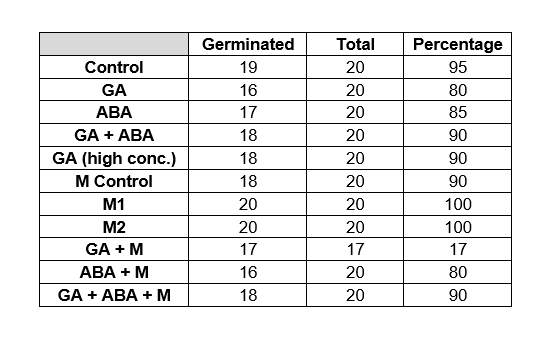
\includegraphics[width = \linewidth]{Number of Seeds Germinated.png}


\begin{comment}
\subsubsection{Shoot Length}
\begin{figure}[H]
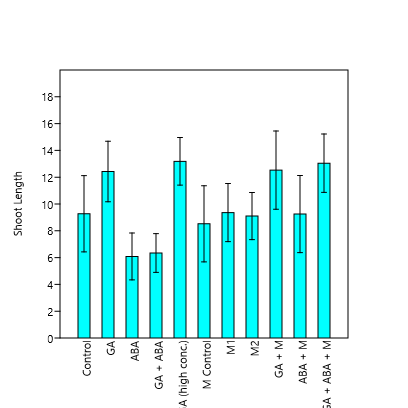
\includegraphics[width = \linewidth]{Shoot Length Barplot.png}
\caption{Shoot Length Barplot with 95\% confidence intervals}
\end{figure}

\subsubsection{Root Length}

\begin{figure}[H]
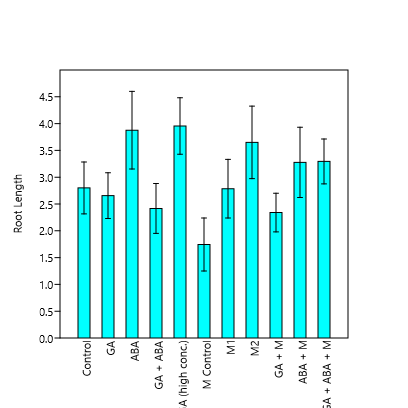
\includegraphics[width = \linewidth]{Root Length Barplot.png}
\caption{Root Length Barplot with 95\% confidence intervals}
\end{figure}

\subsubsection{Shoot/Root Length Ratio}

\begin{figure}[ht!]
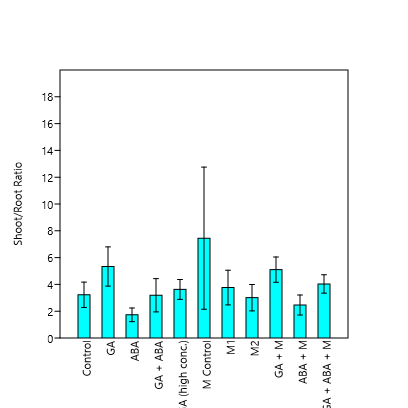
\includegraphics[width = \linewidth]{SR Ratio Barplot.png}
\caption{Shoot/Length Ratio Barplot with 95\% confidence intervals}
\end{figure}
\end{comment}


%\begin{strip}
%\makebox[\linewidth]{\rule{\paperwidth}{0.4pt}}
\section{References}
\begin{itemize}
    \item \href{https://byjus.com/biology/seed-germination/}{Seed Germination - Byjus}
    \item \href{https://www.investopedia.com/terms/n/normaldistribution.asp}{Normal Distribution - Investopedia}
    \item \href{https://stattrek.com/hypothesis-test/hypothesis-testing.aspx}{Hypothesis Testing - Stat Trek}
    \item \href{http://mathworld.wolfram.com/HypothesisTesting.html}{Hypothesis Testing - Wolfram MathWorld}
    \item \href{https://blog.minitab.com/blog/adventures-in-statistics-2/understanding-t-tests-1-sample-2-sample-and-paired-t-tests}{Understanding t-tests - The Minitab Blog}
\end{itemize}
%\end{strip}

\end{document}